% This must be in the first 5 lines to tell arXiv to use pdfLaTeX, which is strongly recommended.
\pdfoutput=1
% In particular, the hyperref package requires pdfLaTeX in order to break URLs across lines.

\documentclass[11pt]{article}

% Remove the "review" option to generate the final version.
% \usepackage[review]{emnlp2021}
\usepackage{emnlp2021}

% Standard package includes
\usepackage{times}
\usepackage{latexsym}

% For proper rendering and hyphenation of words containing Latin characters (including in bib files)
\usepackage[T1]{fontenc}

% This assumes your files are encoded as UTF8
\usepackage[utf8]{inputenc}
\usepackage{microtype}

% ======================================================================
% PEC For some reason the EMNLP templates put LH column line numbers on
% the right side. This switches them to the left side.
\usepackage[switch]{lineno} % default option is 'left
% ======================================================================

% PEC additions
\usepackage{graphicx}
\newcommand{\nk}[1]{\textcolor{green}{Nora: #1}}
\newcommand{\eat}[1]{}
\newcommand{\red}[1]{\textcolor{red}{#1}}
\newcommand{\blue}[1]{\textcolor{blue}{#1}}
\newcommand{\orange}[1]{\textcolor{orange}{#1}}
\newcommand{\green}[1]{\textcolor{ForestGreen}{#1}}
\newcommand{\teal}[1]{\textcolor{teal}{#1}}
\newcommand{\magenta}[1]{\textcolor{magenta}{#1}}
\usepackage{quoting}
\newenvironment{myquote}{                   % list without par spacings
  \parskip 0mm \begin{quoting}[vskip=0mm,leftmargin=2mm]}{
\end{quoting}}
\newenvironment{ite}{                     % list without par spacings
     \parskip 0cm \begin{itemize} \parskip 0cm \parsep 0cm \itemsep 0cm \topsep 0cm}{
        \end{itemize}} %  \parskip 0cm}
\newenvironment{enu}{                   % list without par spacings
     \parskip 0cm \begin{list}{}{\parsep 0cm \itemsep 0cm \topsep 0cm}}{
       \end{list}} %  \parskip 0cm}
\newenvironment{des}{                 % list without par spacings
     \parskip 0cm \begin{list}{}{\parsep 0cm \itemsep 0cm \topsep 0cm}}{
       \end{list}} %  \parskip 0cm}
\newenvironment{myenumerate}{                   % list without par spacings
     \parskip 0cm \begin{enumerate}{\parsep 0cm \itemsep 0cm \topsep 0cm}}{
        \end{enumerate}} %  \parskip 0cm}
\newenvironment{myitemize}{                     % list without par spacings
     \parskip 0cm \begin{itemize}{\parsep 0cm \itemsep 0cm \topsep 0cm}}{
        \end{itemize}} %  \parskip 0cm}

% ======================================================================

% If the title and author information does not fit in the area allocated, uncomment the following
%
%\setlength\titlebox{<dim>}
%
% and set <dim> to something 5cm or larger.

\title{Endowing Language Models with a Notion of Belief (?)}

% Author information can be set in various styles:
% For several authors from the same institution:
% \author{Author 1 \and ... \and Author n \\
%         Address line \\ ... \\ Address line}
% if the names do not fit well on one line use
%         Author 1 \\ {\bf Author 2} \\ ... \\ {\bf Author n} \\
% For authors from different institutions:
% \author{Author 1 \\ Address line \\  ... \\ Address line
%         \And  ... \And
%         Author n \\ Address line \\ ... \\ Address line}
% To start a seperate ``row'' of authors use \AND, as in
% \author{Author 1 \\ Address line \\  ... \\ Address line
%         \AND
%         Author 2 \\ Address line \\ ... \\ Address line \And
%         Author 3 \\ Address line \\ ... \\ Address line}

\author{Nora Kassner, Hinrich Sch{\"u}tze \\
Center for Information and Language Processing \\
LMU Munich, Germany \\
\texttt{kassner@cis.lmu.de} \\ \And
Oyvind Tafjord, Peter Clark \\
Allen Institute for AI \\
Seattle, WA \\
\texttt{\{oyvindt,peterc\}@allenai.org} \\
}

\begin{document}
\maketitle
\begin{abstract}
\nk{Regarding the title: I liked the Believe me...}
Although language models (LMs) \nk{Should we call it pre-trained LM and refer to it as PLMs?} have become adept at question-answering (QA), they
still can produce inconsistent answers, 
% Below - need to acknowledge there's already work on consistency reduction
even after using specialized training techniques to reduce model inconsistency. As a result, it can be hard to identify
% making it hard to identify  - old version
what the model actually
"believes" about the world. Our goal is to reduce this problem, so LMs are 
more globally consistent and accurate in their answers. Our approach is to add a memory
component - a BeliefBank - that records a model's raw 
% answers and improves consistency among them by flipping answers that significantly clash with others.
% NEW
answers; and a reasoning
component - a weighted SAT solver - that improves consistency among beliefs by
flipping answers that significantly clash with others. Thus, the overall system
constructs a more coherent picture of the world from the model's raw answers.
% -- end NEW 
We show that, in a controlled experimental setting, 
% where facts are simple propositions (e.g., "eagles are birds"), 
both accuracy and consistency
is improved. We also show that, by recalling pertinent beliefs from the
BeliefBank as context for new questions, raw answer accuracy for those unseen
questions is also improved. This feeds more accurate answers back into the growing
BeliefBank, creating a dynamic cycle of interaction between the model and BeliefBank.
This is significant as it is a first step towards endowing models with an evolving,
persistent memory, and creating systems that continuously improve over time.
\end{abstract}

\eat{
\red{Why experiments are slow:
\begin{itemize}
    \item calibration is a problem!!! When I extended the dataset the calibration seems to not work well. I changed it to a heuristic alternative which seems to work but that means I have to rerun all SAT solving experiments
    \item SAT solving takes per entity: 6 min
    \item each run of the full graph takes > 1h
    \item + 10 plants: 10 h
    \item + 20 incremental with random context: 20
    \item + 20 incremental with bm25 context: 20
    \item + 20 incremental with bm25 SAT solved context: 20
    \item + averaging over multiple splits maybe 5?: 20*4
\end{itemize}}

\red{What are the current issues:
\begin{itemize}
    \item If calibration is of F1 can still improve but it flips essential things from no-->yes and random things from yes-->no
    \item What kind of F1 should I report? Derivable facts (small test set but large improvements), gold facts (even smaller test set with good model performance and only small improvements, all IsA facts (might include a couple of wrong labels, large test set, only slight improvements as many nodes need more mutual exclusive connectivity)
    \item I have to filter plurals
    \item Do we expect the model to understand negation inside to context window?
\end{itemize}}
}

\section{Introduction}

% \vspace{-1mm}
\begin{figure}[t]
\centering
     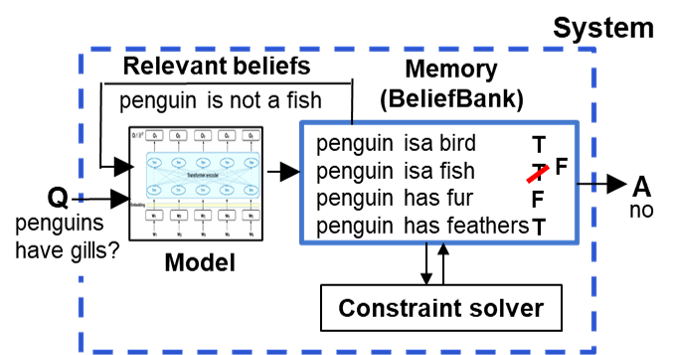
\includegraphics[width=1\columnwidth]{architecture2.png}	   % small figure
%      \vspace{-3mm}
\caption{The proposed architecture. The model's raw answers are stored in a
persistent memory (BeliefBank), and potentially flipped if they clash
significantly with others. Pertinent beliefs are then used to help the model answer new
questions. We find the consistency and accuracy of both the model and the overall
system improves with time. \label{architecture}}
% \caption{The proposed architecture. A memory layer (the BeliefBank)
% plus constraint solver improves the consistency of beliefs.
% Given a new question, relevant beliefs are recalled to help improve
% the model's answers, thus feeding more accurate results back into the BeliefBank.
% \label{arcuitecture}}
% \vspace{-3mm}
\end{figure}

How might we ascribe a notion of belief to a model? Prior work has shown that, while
models have high question-answering (QA) accuracy \nk{should we specify that we are talking about “closed-book question answering” and refer to papers that show that PLMs are good at it? }, they can also be inconsistent in their
answers, making it hard to pin down what a model actually ``believes'' about a proposition.
Our goal is to reduce this problem by having systems provide more globally consistent
answers to questions.

Prior work on reducing inconsistency has focused on retraining the model itself to be
more consistent in its answers, e.g., \cite{Ribeiro2019AreRR,Li2019ALF}, but with imperfect results. We present an
alternative approach in which the model is unchanged, but an evolving, persistent memory
of beliefs - called the BeliefBank - is layered on top, and a reasoning component - a
weighted SAT solver - is used to improve consistency among beliefs. 
Thus, the overall system attempts to build a more coherent representation of the
world from the model's raw answers, by ruminating on the answers seen so far.
This can be viewed as assembling a simple ``mental model'' of the world from
the noisy output of a raw LM. 

Just as the model helps populate the BeliefBank, we also show how beliefs in
the BeliefBank can improve the model's answers to future questions,
by using the most relevant beliefs as additional context for question-answering
(i.e., reminding the model of important facts pertinent to the new question).
These improved answers then feed into the growing BeliefBank, allowing the
overall system (model + BeliefBank) to continuously improve performance over
time, without retraining the model itself.

We explore this in a controlled experimental setting where 
both candidate facts and candidate constraints are provided. Candidate facts are simple
sentences that may be true or false, e.g., "An eagle is a bird" (T), ``An eagle is a mammal'' (F). Candidate constraints are between (variabilized) facts, e.g., ``?X is a bird $\rightarrow$ ?X can fly''. These allow us both to probe and measure improvement
in the system's consistency and accuracy, described shortly.

\eat{
\red{Delete/reword this paragraph} Our approach involves an interplay between a model's raw answers, and an
evolving memory - the BeliefBank - of beliefs based on the model's earlier answers
and a set of constraints that should hold. Model's answers contribute to the BeliefBank,
and the BeliefBank contribute new context to help with future question-answering by
the model. In between, a constraint system serves to identify and reduce inconsistency
among beliefs in the BeliefBank. Combined, this results in a system capable of
continuous improvement over time, opening new possibilities for dialog and
interactive teaching.
}

\red{List contributions}

\section{Related work}

While there has been some prior work on improving answer consistency, the primary approach
has been through modified model training. \citet{Ribeiro2019AreRR} improved consistency
by adding question paraphrases and question implications to the training data (data augmentation).
Others have trained models with (small) {\it sets} of examples with known constraints
between them, and included an additional loss term reflecting inconsistency among
set members during training \cite{Minervini2018AdversariallyRN,Li2019ALF,Asai2020LogicGuidedDA}.
However, the constraints are unused at test time (beyond what the model may have
internalized), and inconsistent answers are still produced.

For problems requiring a structured answer, e.g., predicting a sequence of
state changes, domain-specific constraints have been used to downgrade/block
answers that violate them \cite{Tandon2018ReasoningAA,Du2019BeCI}. This
encourages consistency within a single answer structure, but not among
different answers, our goal here.

% Concerning improving global consistency using constraints,
In the area of knowledge graph construction
% , where individual extractions may be noisy, 
\citet{Pujara2013KnowledgeGI} define ``knowledge graph identification''
as the task of building a maximally consistent knowledge graph given noisy facts
and their extraction confidences, and ontological constraints between them.
They develop a solution use probabilistic soft logic (PSL) \cite{Broecheler2010ProbabilisticSL}
as their constraint reasoner. 
Similarly \citet{berant2010global} learn the globally
optimal set of entailments between a large database of candidate
entailment pairs (with associated confidences), by applying
a global transitivity constraint (X$\vdash$Y \& Y$\vdash$Z $\rightarrow$ X$\vdash$Z)
using Integer Logic Programming. 
Our constraint solver performs an analogous
function in our architecture, using the Z3 SAT solver (Section~\ref{??}).
\red{Say how we are different/go beyond.}

An important part of our contribution is the use of a dynamic, persistent memory.
While there are neural architectures that include an associated memory,
e.g., \cite{Henaff2017TrackingTW,Sukhbaatar2015EndToEndMN}, these components
typically play the role of a short-term working memory to help computation.
In contrast, our BeliefBank memory layer is a persistent, long-term memory of
explicit beliefs.


\nk{some more related work to add:
Prior work analyzing knowledge captured by pre-trained LMs 
add: inconsistency with respect to knowledge captured by pre-trained LMs paraphrases, grammatical number and negation \cite{Elazar2021MeasuringAI, ravichander-etal-2020-systematicity, ettinger-2020-bert, kassner-schutze-2020-negated}. 
2 more inconsistency papers: \citet{Camburu2020MakeUY}
\citep{du2019consistent}
}
% \red{Possibly cite \cite{Graves2016HybridCU} - the memory there is more like
% an opaque expansion of the original network. I'm inclined not to cite this though
% as it's old and not really relevant.}

% \subsection{PLMs and knowledge}
\subsection{Faithfulness}
\citet{subramanian-etal-2020-obtaining}
introduce the concept of module-wise faithfulness, a systematic evaluation of faithfulness in neural module networks for reasoning. We show that naive training does not produce faithful modules and propose several techniques to improve module-wise faithfulness. 

\subsection{Inconsistencies in KGs}
(copied from old paper, need rewrite)
Consistency in KBs has been
studied in theoretical frameworks in the context of the
satisfiability problem and KB construction, and efficient
algorithms for detecting inconsistencies in KBs have been
proposed \cite{hansen2000probabilistic,andersen2001easy}.
Other work aims to quantify the degree to which KBs are
inconsistent and detects inconsistent statements
\cite{Thimm:2009d,muino2011measuring,Thimm:2013}.
\cite{zhang2020need} showed that capturing factual knowledge inside PLMs is a specially resource hungry task.





\section{Task}

\subsection{Beliefs}

What does it mean to believe a proposition, say p = eagles are birds? In general, a system can
be said to (appear to) believe something if it acts as if it were true. In the specific
context of a QA system, we would expect it to produce answers consistent with p (and
its other beliefs). Pragmatically, we expect the system to (a) give a consistent answer to
different paraphrases of the question "p?" ("Are eagles birds?", "Is an eagle a type of bird?", ...),
and (b) give correct answers about implications of p ("Eagles lay eggs", "Eagles have feathers", ...),
conditional on the system knowing such implications and how to apply them.
% For example,
% if a system believes eagles are birds, and knows birds lay eggs (plus the rule of inheritance),
% we would expect it to answer "yes" to a question about whether eagles lay eggs.
Of course, a system may not perfectly answer such implications as the implications
may have exceptions, or the system may not be a perfect reasoner.\footnote{Similarly,
people do not always behave fully consistently with their professed beliefs.}.
Thus, to the external observer, there are {\it degrees} to which a system acts as if it
believes something.
% (Note this is distinct from a system's internal confidence in a belief).

\eat{
\red{Possibly delete this paragraph if too repetitive.} 
As has been shown elsewhere, language models (LM) can be inconsistent in their answers,
suggesting they have a rather weak notion of belief, in the sense described above.
To strengthen this, we add a dynamic memory component - the BeliefBank - on top of
the model to track and modify beliefs. We use the phrase ``the {\bf system}'' to refer
to the combined model plus belief bank. Our goal is to create a system with
a stronger notion of belief (i.e., more consistent and accurate) than the underlying LM inside it.
}

\subsection{Task Definition}

Our goal is to ascribe a stronger notion of ``belief'' to a system that includes a model $M$,
by improving the consistency and accuracy of its answers (compared with $M$). To measure
this we consider a true/false QA task, where we are also given a set of
constraints between answers:
\begin{myquote}
{\bf Given:}
\begin{ite}
\item a set of {\bf sentences} $S$ 
\item a set of {\bf constraints} $C(S)$ between (the truth values of) sentences in $S$, each annotated with a penalty $p_i$ to apply if $c_i$ is violated
\item a {\bf model} $M$ that takes as input a True/False (NL) question $Q$ and (NL) context $X$, and predicts a True/False answer $A$ with confidence score $F$
\end{ite}
{\bf Predict:}
\begin{ite}
\item the True/False labels for $S$, so as to maximally improve accuracy (with respect to gold labels) and
   consistency (minimize total penalties of constraint violations) compared with model $M$'s raw answers
\end{ite}
\end{myquote}
As our dataset class distribution (described shortly) is unbalanced, with significantly fewer True than False
answers, we measure accuracy using F1 (over True questions) to avoid scores being dominated by negative
answers.



\section{Approach}

Our goal is to ascribe a stronger notion of ``belief'' to a model,
by improving the consistency and accuracy of its answers. Our approach is to add a
memory layer, called the {\bf BeliefBank}, on top of the model to track and modify
beliefs. We evaluate two methods for leveraging the BeliefBank:
\begin{des}
\item[{\bf Constraint solving:}] Given a model $M$'s answers (with confidences) in the BeliefBank, a constraint
solver seeks to reduce constraint violations by potentially flipping answers that maximally clash
with other answers. The answers in the revised BeliefBank are taken as the system's {\it overall} answers
to questions.
\item[{\bf Feedback:}] Given a new question $q_{n}$, relevant beliefs in the BeliefBank are
provided as additional input (namely as context) to help it answer $q_{n}$,
to see if this improves the model's answer.
\end{des}
Figure~\ref{architecture} illustrates this architecture.

\subsection{Definitions \label{definitions}}

\noindent Let
\vspace{-2mm}
\begin{ite}
 \item a {\bf belief} $b_i$ = a triple ($s_i$,$b_i$,$c_i$), where
    \begin{ite}
     \item $s_i$ is a sentence $\in S$ % expressing a proposition about the world
     \nk{we should not call the belief and the truth of $s_i$ both $b_i$}
     \item $b_i \in$ \{T,F\} denotes the system's belief about the truth of $s_i$
     \item $w_i$ is a number 0-1 representing the system's confidence in that belief
    \end{ite}
 \item a {\bf BeliefBank} $B(S)$ = a set of beliefs over sentences $S$ = $s_1,...,s_n$
 \item For notational convenience, we denote the believed truth $b_i$ of $s_i$ according to $B(S)$ as $bel(s_i,B(S))$
 \item a {\bf constraint} $c_i$ = a 4-tuple of the form
\begin{myquote} \centering
($if_i \rightarrow then_i, tf_i, p_i$)
\nk{It took me some time to see what is going on here. I think it is comfunsing to call it $if_i$. On first glance it does not read as if but as an index i then f and then again index i...}
\end{myquote} 
where $if_i, then_i$ are sentences, e.g., \\
\vspace{1mm}
\hspace*{1mm} ``A poodle is a dog'' $\rightarrow$ ``A poodle has a tail'' \\
\vspace{1mm} 
and $tf_i \in$ \{True,False\} denotes, if $if_i$ is true, the expected truth of $then_i$ (here, True),
with penalty $p_i$ if it is not.
\item A {\bf constraint graph} $C(S)$ = a set of constraints $c_i$ over sentences $S$
\end{ite}
Given a set of beliefs $B(S)$ about $S$ and a set of constraints $C(S)$, we define the {\it consistency}
of those beliefs as (the negative of) the total penalty of violated constraints.
Dropping the $S$ parameter for convenience:
 \begin{myquote}
  consistency(B,C) = \\
\hspace*{2mm}  $- \sum_{c_i \in C} \{~ p_i ~ | ~ c_i = (if_i \rightarrow then_i, tf_i, p_i )       ~\& \\
\hspace*{18mm}  bel(if_i,B) ~ \& ~ bel(then_i,B) \neq tf_i~ \}$
\end{myquote}
Although this measure is dependent on the constraints and penalties used,
it allows us to perform {\it comparative} experiments with different systems.

\begin{table*}
\centering
{\small
\begin{tabular}{|l|ll|ll|ll|ll|} \hline
Results after seeing $\rightarrow$ & \multicolumn{2}{|c|}{\bf batch1} &
\multicolumn{2}{|c|}{+ {\bf batch2}} &
\multicolumn{2}{|c|}{+ {\bf batch3}} &
\multicolumn{2}{|c|}{+ {\bf batch4} (all)} \\
Accuracy (F1), Consistency $\rightarrow$ & F1 & Con & F1 & Con & F1 & Con & F1 & Con \\ \hline           
model (raw) & 48 & 76 & 28 & 79 & 42 & 75 & 44 & 72\\
model + constraints & & & & & & & & \\
model + feedback (bm25) & 48 & 76 & 39 & 92 & 48 & 78 & 58 & 86\\
model + feedback (random) & 48 & 76 & 42 & 94 & 56 & 86 & 56 & 81\\
model + constraints + feedback (most confident) & & & & & & & & \\
model + constraints + feedback (relevant for query) & & & & & & & & \\
model + constraints + feedback (relevant for query + flipped) & & & & & & & & \\\hline
bm25 with most confident ones?\\
\end{tabular}
}
\caption{{\bf model (raw)} shows the accuracy (F1) and consistency (Con) of the
model stand-alone, after each batch of questions. 
 In {\bf model + constraints}, the constraint solver is run
 after each batch on all the answers seen so far. In {\bf model + feedback},
 questions in batch2 are posed to the model along with selected beliefs from
 all earlier batches (batch1), but the constraint solver is unused. 
 {\bf model + constraints + feedback} is the same, except the constraint solver is also run
 after each batch on all answers seen so far.
\label{incremental-improvement}}
\end{table*}

\subsection{Methods}

\subsubsection{Constraint Solving}

Given a set of beliefs and constraints, the constraint solver has two competing objectives: (a) flip 
beliefs so as to minimize constraint penalties (b) don't flip beliefs, so as to preserve
the model's raw predictions. We balance these two objectives with a hyper-parameter:
\begin{quote}
    Equation here
\end{quote}

To find the optimal solution to the constraint equations, we convert the problem into a weighted SAT problem,
and then use the Z3 SAT solver to find the optimal truth assignments to the beliefs. \red{Details are in
Appendix~\ref{??}}.

\subsubsection{Feedback}

Given a new question $q_i$ and set of beliefs $B$, we augment
$q_i$ with a {\it context} containing the beliefs most relevant to $q_i$
before posing it to the model. Our conjecture is that if the 
model is explicitly reminded of relevant beliefs when answering a new question,
it will answer the question more accurately and consistently.

We evaluate three policies for chosing which beliefs to feed back to $M$:
\begin{enu}
\item[1.] randomly selected from $B$
\item[2.] most similar, using the BM25 information retrieval ranking function \cite{bm25}
\item[3.] most confident (``core'') beliefs about the queried entity $e$, ... \red{explain}
\end{enu}
In all cases, three beliefs are selected.

\section{Dataset}

We create a dataset to test our approach in a controlled way, allowing us to perform systematic experiments to evaluate behavior.

\subsection{Constraint Templates}
\nk{I think the terms "constraint templates" and "sentence templates" are confusing. I would call them simply constraint and either sentence/assertion or query. And use the word template for the query template, e.g. Is X a Y?.}
A {\bf constraint template} $t_i$ is a generalized constraint, namely a 4-tuple of the form
\begin{myquote} \centering
($if_i \rightarrow then_i, tf_i, p_i$)
\end{myquote} 
where $if_i, then_i$ are sentences containing a single, shared variable ?X, e.g.,
\begin{myquote} \centering
\nk{I would prefer simply using X instead of ?X}
``?X is a dog $\rightarrow$ ?X has a tail.''
\end{myquote}
If $if_i$ is true, then $tf_i \in$ \{True,False\} denotes the expected truth of $then_i$, 
with penalty $p_i$ if it is not.

\noindent
The dataset contains two kinds of constraints:
\begin{des}
\item[{\bf positive implications:}] ($tf_i$ = True), e.g.,``?X is a dog $\rightarrow$ ?X has a tail.''
\item[{\bf mutual exclusivity:}] ($tf_i$ = False), e.g.,
``?X is a dog $\rightarrow$ [$tf$=FALSE] ?X is a bird.'',
and ``?X is a bird $\rightarrow$ [$tf$=FALSE] ?X is a dog.'', to
express that an entity cannot be both a dog and a bird at the same time.
% These are expressed as a pair of constraint templates each with $tf_i$ = False:

\end{des}
Positive implications were gathered from a filtered subset of ConceptNet triples involving the 6 relations: IsA, HasA, MadeOf, PartOf, HasProperty, CapableOf. For example, the ConceptNet triple (dog, HasA, tail) gives rise to the constraint ``?X is a dog $\rightarrow$ ?X has a tail.''. We only consider ConceptNet triplets with weights larger than 1.0 

Triples were filtered

by \red{describe filtering method here}.

Mutual exclusivities were gathered from a filtered subset of the WordNet taxonomy,
based on the approximation that (generally) siblings in the WordNet noun hierarchy
are mutually exclusive \red{elaborate}.

We collected 13,000 constraint templates in this fashion (3k implications, 10k mutual
exclusivities).

\subsection{Constraint Violation Penalties}

We used a combination of crowdsourcing and calibration to assign a reasonable
constraint violation penalty $p_i$ to each constraint. Workers were shown each
template and asked to judge if the implication held always/usually/sometimes/rarely/never with raw scores 4/3/2/1/0.
Three workers independently scored each template and the scores averaged.
The raw scores were then calibrated by sigmoid-scaling \red{against what gold data?}, using a
grid search over slope and shift to identify the scaling hyper-parameters.

\subsection{Sentence Templates}
\nk{I am not sure what this passage is referring to? I have templates for the assertions? You call these assertion sentence, right? I have for each relation a different template. As there are 6 relations I have 6 templates. Why 200?}
We collect all the unique variabilized sentences in the constraints together,
resulting in 200 \red{??} sentence templates, e.g., ``?X is a dog.''.

\subsection{Facts and Constraints}
\nk{Not sure about this section name. }
Given the sentence and constraint templates, we can create a {\bf grounded} slice of
data by instantiating ?X with a particular entity, e.g., ``poodle'' (resulting in 200 
sentences and 13000 constraints about poodle). To assign True/False labels to the
sentences, we identify and manually annotate the leaf sentences in the constraint DAG,
and then use the constraint rules to infer True/False labels for other sentences.
This provides ``silver'' labels for all the sentences, silver because constraint
rules may have exceptions in the real world for particular individuals (e.g.,
penguins don't fly). For a given slice, we denote the sentences as $S$ and
the constraints about them as $C(S)$.

We repeat this for 120 \red{??} entities (100 animals, 20 plants), resulting
a final dataset containing {\bf ?? silver facts} (sentences + True/False labels) and {\bf ?? constraints}
(120 slices $\times$ 200 facts and 1000 constraints).
Note that each slice is independent and can be processed separately.
As described shortly, we perform our experiments with each slice in turn
and average results.

\subsection{Dataset Split}

We randomly split each slice into four batches (batch1, batch2, batch3, batch4) to measure
improvement with time, shown later.

\section{Model}

The fixd model $M$ that we use for our experiments is the multi-angle QA system MAQAw \cite{arc-da}.
MAQAw is a derivative of UnifiedQA, a state-of-the-art T5 model fine-tuned on $\approx$400k question-answer pairs.
MAQAw was then 
further fine-tuned on several thousand science questions and trained on different permutations of inputs and outputs
(e.g., question Q + context C $\rightarrow$ answer A; CA $\rightarrow$ Q; etc.). MAQAw outputs an answer probability...
NOTE this model is fixed for our experiments here.

\section{Experiments}

We present the results of three sets of experiments in this environment:
\begin{enu}
\nk{Not sure about the naming here. Let's discuss!}
\item[{\bf 1. Model:}] How accurate and consistent is the model, a priori?
\item[{\bf 2. Model + BeliefBank:}] To what extent does adding a BeliefBank memory layer improve the consistency and accuracy
           of the overall system (model + BeliefBank)?
\item[{\bf 3. Model + BeliefBank + Feedback:}] Can we use the beliefs in the BeliefBank to improve {\it future} answers by the model
to new (unseen) questions?
\end{enu}

% Given a set of questions $q1,...,q_n$ about sentences $S$, we can pose them to $M$ and collect both the answers (True/False)
% and confidences to form the raw model's beliefs $B_{model}(S)$ about $S$.

\subsection{Model}

How accurate and consistent is the model, a priori?

We evaluate the model's consistency and accuracy for ? different data groups (entities). The results are shown in Table~\ref{??}.

Results show models aren't perfectly consistent in their beliefs.

\subsection{Model + BeliefBank}

% The model alone is inconsistent in its beliefs, making it hard to identify what its ``opinion'' is.

We now attempt to do better, by adding a memory (a BeliefBank) plus a reflective component (a constraint solver)
to the overall system. By ruminating on the model's raw beliefs, the constraint solver may determine
that some beliefs should be flipped based on the weight of evidence from other beliefs. We refer
to the combination of the model plus memory (BeliefBank) as ``the system'', whose beliefs are those
in the maintained BeliefBank.

Results show that the constraint solver improves both the consistency and correctness
of the system's beliefs.

% \begin{figure}[t]
%\centering
%     \includegraphics[width=1\columnwidth]{architecture.png}	   % small figure
%\caption{The model's raw answers are stored in a persistent memory (BeliefBank),
%and potentially flipped if they clash significantly with others. Pertinent
%beliefs are then used to help the model answer new questions. We find both
%consistency and accuracy of the overall system improves. \label{architecture}.}
% \vspace{-3mm}
%\end{figure}

\subsection{Model + BeliefBank + Feedback}

Can we use the beliefs in the BeliefBank to improve answers to {\it new} questions by the model?
To do this, given a new question, relevant beliefs are used as 
context to the model for question-answering, as illustrated in Figure~\ref{architecture}. 
By reminding the model of corrected or salient beliefs, we conjecture that the model itself
will improve its question-answering ability, in turn potentially improving the
BeliefBank.

We evaluate three policies for selecting relevant beliefs for a new question:
\begin{des}
\item[(a)] The top 10 beliefs most similar to the question, as identified by BM25 (information retrieval)

\item[(b)] The top 10 {\it corrected} beliefs (i.e., only use beliefs that the model was originally mistaken about)
\item[(c)] The top 10 {\it positive, corrected} beliefs (i.e., ignore negative ``It is not the case tha...'' beliefs).

\item[(d)] The top {\it most confident beliefs} independent of if they have been corrected or not. (running)
\item[(e)] The top {\it most relevant beliefs} defined by the constraint graph
\end{des}

Baselines:
\begin{des}
\item[(a)] 3 random beliefs of the model without SAT: works better than bm25 as it has more variety in what it adds whereas bm25 if no good match is found add always the same unhelpful context.
\item[(b)] The top 3 beliefs most similar to the question, as identified by BM25 (information retrieval) without SAT: see (a)
\item[(c)] 3 random beliefs of the belief bank after SAT.
\item[(d)] 3 most confident assertions according to the constraints: This works if the relevant queries have been already asked, if not it has the same problem as bm25 as it then adds always the same unfortunate context.
\end{des}
% Given the new answer, we run the constraint solver as usual. We are interested in whether
% an improved model (using one of these policies) + constraint solver will outperform a fixed
%  model + constraint solver.

To evaluate performance on a new, unseen questions,
we divide the dataset randomly into four batches.
% , and incrementally provide each
% batch to the overall system (rather than evaluate incrementally for every instance).
First the model answers all questions in $batch_1$ with no context, and the BeliefBank
is created and updated using the constraint solver. Then, the model answers all
questions in $batch_2$ with a context provided from the BeliefBank ($batch_1$) questions,
and the constraint solver rerun. We similarly repeat for $batch_3$ and $batch_4$.
Results are shown in Table~\ref{incremental-improvement}.

\section{Discussion and Expansion}

What's needed to take this to real QA? 
\begin{ite}
\item Beyond triples
\item Sources of constraints
\item Source of queries (e.g., which questions should we ask)
\item Resource-bounded constraint solving (e.g., explore just to depth D)
\end{ite}

\section{Conclusions}

\section*{Acknowledgements}


% Entries for the entire Anthology, followed by custom entries
\bibliography{anthology,custom}
\bibliographystyle{acl_natbib}

\end{document}


\subsection{contributions}
\begin{itemize}
    \item rule dataset
    \item mutual exclusive rules are not well captured by the model
    \item ConcepNet rules are captured but not consistently applied
    \item common sense knowledge base identification from a noisy PLM/ mechanism to compose rules and assertion to improve F1 and consistency
\end{itemize}
\section{Data}
Rules are generate from ConcepNet \cite{Speer2017ConceptNet5A}.
Relations: IsA, CapableOf, HasParts, HasProperty, MadeOf, HasA.

Two types of rules: transitive rules and mutual exclusive rules.

Subjects from WordNet \cite{wordnet}.
\section{Calibration}
\section{Results}
\subsection{Consistency}
\begin{table*}
\begin{tabular}{ l|c|c} 
& consistency model & consistency resolved \\\hline
transitive rules & & \\\hline
mutual exclusive rules & & \\\hline
both & & \\\hline
\end{tabular}
\caption{Consistency before and after wSAT solving}
\end{table*}
\subsection{Accuracy}
\begin{table*}
\begin{tabular}{ l|c|c} 
& F1 model & F1 resolved \\\hline
gold facts & \\\hline
deducible facts& \\\hline
non-deducible facts&& \\\hline

\end{tabular}
\caption{F1 before and after wSAT solving model rules.}
\end{table*}
\subsection{Model rules vs. gold rules}
\subsection{Incremental}
\subsection{Self diagnosis}
Identifying regions where more rules are needed or where model rules need human intervention.
\section{Related Work}

